In the previous chapter,
  we introduced the concept
  of a {\em simulation entity\/},
  with type \lstinline|SimEntity|,
  as being the predominantly interesting object
  in a discrete-event simulation.
In the current chapter,
  we narrow this down to 
  the use case of {\em queueing systems},
  and we introduce {\em jobs},
  with type \lstinline|SimJob|,
  and {\em queues},
  with type \lstinline|SimQueue|,
  as the most interesting manifestations
  (specializations if you will) of
  a \lstinline|SimEntity|.

Our strategy in describing both
  \lstinline|SimJob| and \lstinline|SimQueue|
  in this chapter
  is to introduce their structure
  (properties) and behavior (operations and notifications)
  in a concise manner,
  using the foundation laid in Section \ref{chap:entities},
  without elaborating into examples.
We believe that both concepts are best understood
  when presented in a compact yet complete form.
Moreover,
  we cannot introduce examples without
  concrete implementations of
  \lstinline|SimJob| and \lstinline|SimQueue|.
    
\section{Visits, Arrivals and Departures}

The central notion in \lstinline|jqueues|
  is that a queueing-system simulation (run)
  consist of a sequence of {\em visits\/}
  of entities named {\em jobs},
  \lstinline|SimJob|s,
  to others named {\em queues},
  \lstinline|SimQueue|s.
A \lstinline|SimJob| can visit
  {\em at most one\/}
  \lstinline|SimQueue|
  at a time
  but there can be an arbitrary amount of
  (simulation) time
  between successive queue visits.
A \lstinline|SimJob|
  may revisit the same \lstinline|SimQueue|
  arbitrarily many times,
  provided that, obviously,
  these visits do not mutually overlap
  in time.
  
The \lstinline|SimQueue| currently visited by a \lstinline|SimJob|
  ---if any---
  is maintained in the job's
  \lstinline|queue| state property.
If the job is not currently visiting
  a queue,
  the property value is \lstinline|null|.
Likewise,
  the set of \lstinline|SimJob|s currently
  visiting a particular \lstinline|SimQueue|
  is maintained in that queue's
  \lstinline|jobs| state property.
We refer to the "area" holding visiting jobs
  in a \lstinline|SimQueue| as its {\em visit area}.
If no job is currently visiting the queue,
  the latter's \lstinline|jobs| property
  value is the empty set.
  
Since both \lstinline|SimJob.queue|
  and \lstinline|SimQueue.jobs|
  are state properties,
  they are under well-defined
  control of the operations
  on the respective entities.
The most important operations
  are the {\em arrival\/} of a job at a queue.
  and the {\em departure\/} of a job at a queue.
Both will sound familiar to readers with
  some background in queueing theory.
  
In \lstinline|jqueues| release 5,
  the only way to initiate\footnote{We carefully avoid using 'start'
  in this context, in order to avoid confusion later on.}
  a visit is through invocation of the \lstinline|Arrive|
  operation,
  which is external (and thus, user-schedule-able)
  on both \lstinline|SimJob| and \lstinline|SimQueue|.
It is a {\em binary operation\/};
  you can invoke it on any of the two entities
  (job or queue),
  providing the other entity as argument.
The corresponding sub-notification type
  is \lstinline|ARRIVAL|.

If the visit ends "normally",
  i.e.,
  the visiting \lstinline|SimJob|
  has obtained its required service
  or some other requirement is met,
  the \lstinline|SimQueue|
  invokes its internal \lstinline|Depart|
  operation,
  with corresponding sub-notification type
  \lstinline|DEPARTURE|.
Both the \lstinline|ARRIVAL| and \lstinline|DEPARTURE|
  sub-notifications provide the
  \lstinline|SimJob| and \lstinline|SimQueue|
  as argument to (entity) listeners
  in the \lstinline|STATE_CHANGED| notification,
  see Section \ref{sec:entities:notifications}.
  
In Figure \ref{fig:ArriveDepart},
  we show the partial state of
  a \lstinline|SimQueue|
  and \lstinline|SimJob|s that visit it.
(In subsequent sections,
  we will extend this figure until it finally
  captures all state properties and operations
  on a \lstinline|SimQueue|.)
  
\begin{figure}[!htbp]
  \label{fig:ArriveDepart}
  \caption{Arrivals and departures at a \texttt{SimQueue}.}
  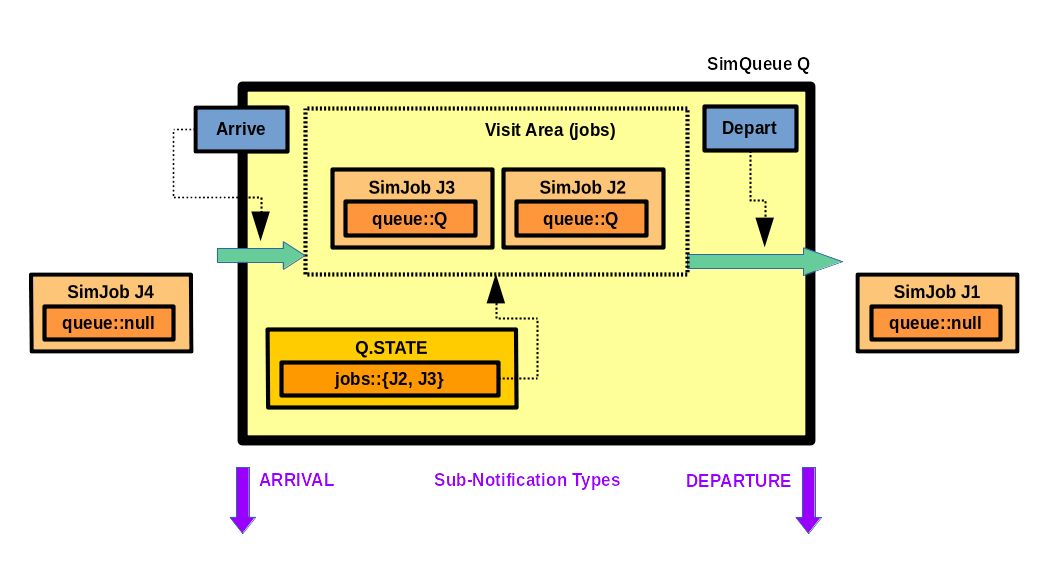
\includegraphics[width=\textwidth]{fig/ArriveDepart}
\end{figure}
    
In the figure,
  jobs \lstinline|J2| and \lstinline|J3|
  are currently visiting \lstinline|SimQueue Q|;
  job \lstinline|J1| just departed from \lstinline|Q| and
  \lstinline|J4| is about to arrive at \lstinline|Q|.
On \lstinline|Q|,
  the \lstinline|jobs| property equals \lstinline|{J2, J3}|;
  the set holds the jobs in its visit area.
Both \lstinline|J2| and \lstinline|J3| have their
  \lstinline|queue| property set to
  \lstinline|Q|;
  on the other jobs it is set to
  \lstinline|null|.
The latter is obviously a prerequisite for jobs to
  be able to arrive at any queue.

The concept of a visit of a job to a queue is
  fundamental in queueing theory,
  and we believe we have captured its most generic
  aspects in \lstinline|SimJob| and \lstinline|SimQueue|:
  a job arrives at a queue for a visit through
  whatever means; we are not concerned with the
  reason of the visit, nor with the nature of
  the "service" that the queue will give to the job.
All we care about is the fact that the job arrives at
  a certain time, and, at the discretion of the queue at hand,
  departs from it at some later time, or even immediately.
The only real constraint we have set is that a job
  can visit at most one queue at a time,
  but this fits, to the author's knowledge,
  most use cases of queueing systems.
  
We want to stress that the only way in which
  to initiate a visit of a job to queue
  is through scheduling an \lstinline|Arrive|
  operation on the event list;
  neither a job nor a queue will
  ever schedule that event by itself.
This means that arrivals can never
  be used by a \lstinline|SimQueue|
  implementation as a means
  to obtain its specification.  
But if \lstinline|Arrive| is invoked
  on a queue that already holds the job provided,
  or if the job is already visiting another queue,
  an \lstinline|Exception| is thrown.
  
Unlike the case with arrivals,
  a departure is {\em not\/} the only
  means by which a visit can end.
In sections further on,
  we introduce {\em dropping},
  {\em revoking\/}
  and {\em auto-revoking}
  a job as alternative means in
  which a queue visit can end.
We then briefly describe
  the case in which
  a visit {\em does not end at all},
  by explaining so-called {\em sticky jobs}.
However,
  before doing that we need to elaborate
  on the {\em partitioning\/}
  of the visits area
  into two separate areas.

\section{The Waiting and Service Areas
         and the \texttt{\bf Start} Operation}
\label{sec:guided:wait-serv-area}

In \lstinline|jqueues|,
  the visit area of every \lstinline|SimQueue|
  is partitioned into
  a {\em waiting area\/} and a {\em service area};
  visiting jobs are always present in precisely
  one of them.
Upon arrival, jobs always enter the waiting area.
At the discretion of the \lstinline|SimQueue|,
  the may move from the waiting area to
  the service area through the internal
  \lstinline|START| operation.
An important and perhaps non-intuitive restriction
  is that {\em jobs cannot move back from the service area
  into the waiting area}.
Note that jobs may depart from either area.
A \lstinline|SimQueue| maintains the
  visiting jobs present in the waiting and service areas
  in its \lstinline|jobsInWaitingArea|
  and \lstinline|jobsInServiceArea| state properties,
  respectively.
Both properties are typed as
  \lstinline|Set|s of \lstinline|SimJob|s.
  
In figure \ref{fig:ArriveDepartStart},
  we illustrate the partitioning of the
  visit area into a waiting area and
  a service area.
  
\begin{figure}[!htbp]
\label{fig:ArriveDepartStart}
\caption{The waiting and service areas of
         a \texttt{SimQueue} and its \texttt{Start} operation.}
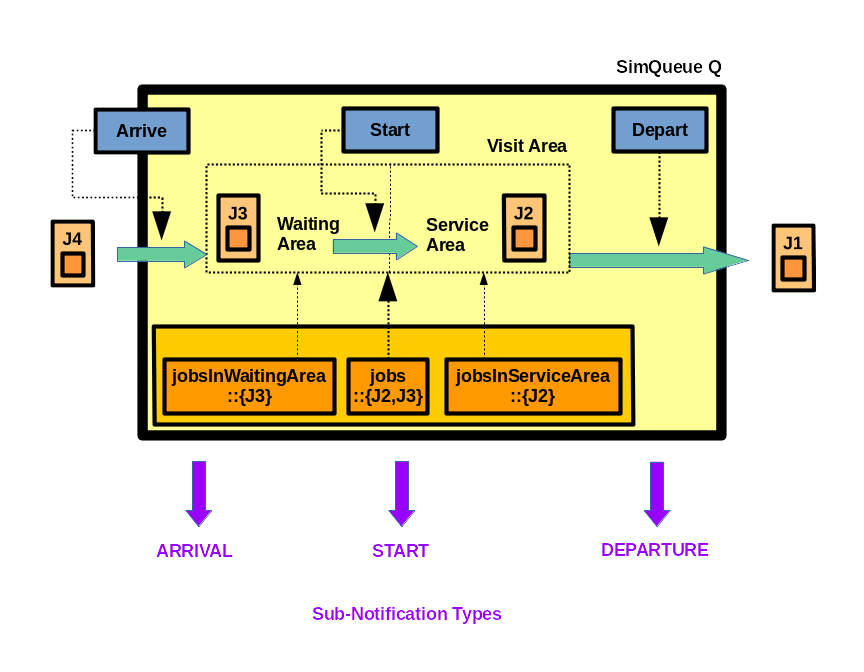
\includegraphics[width=\textwidth]{fig/ArriveDepartStart}
\end{figure}

In the figure,
  jobs \lstinline|J3| is in the waiting area,
  as mandated by the queue's
  \lstinline|jobInWaitingArea|
  (state) property.
Likewise,
  job \lstinline|J2| is in the queue's service area,
  in other words,
  it has {\em started},
  and it is in the queue's
  \lstinline|jobsInServiceArea|
  set.
  
The model for queues in terms of waiting and service area is,
  admittedly, somewhat deviant from models in literature.
The main point is that we make {\em no\/} assumptions
  whatsoever on the structure of the waiting and service areas.
But for most known queueing systems,
  the waiting area is simply a queue holding waiting jobs,
  often in FIFO (First-In First-Out) order,
  and the service area consists of one of more servers
  serving jobs until completion.
In (classical) processor-sharing queues,
  there is virtually no waiting area,
  as jobs enter the service area immediately.

The most obvious complications with this partitioning
  compared to "classical approaches and viewpoints"
  is that since jobs cannot move back from the service area
  into the waiting area,
  one has to let go of the intuitive notion that
  jobs in the service area area actually {\em being served}.
Although true for many queueing systems,
  it is false for systems
  like Preemptive/Resume Last-Come First-Served
  (\lstinline|P_LCFS|),
  and many other preemptive queueing systems.
In \lstinline|P_LCFS|,
  whenever a job in the service area is preempted
  in favor of a new arrival,
  the former stays in the service area,
  yet it is not {\em served\/}
  (at least, not for a while).
Another complication,
  actually induced by \lstinline|jqueues| itself,
  is that in order to start a job,
  a queue needs at least one so-called
  {\em server-access credit},
  but by default this is always the case;
  it is explained in more detail
  in Section \ref{sec:guided:sac}.

\section{The \texttt{\bf Drop} Operation}
\label{sec:drop}
            
In the previous sections
  we noted that the "usual" means in
  which a visit ends
  (after the visiting job has acquired all it needs from the queue)
  is through the \lstinline|Depart| operation.
However, a \lstinline|SimQueue| may decide
  that these requirements cannot or can no longer be met
  due to queue-specific {\em constraints},
  and that the job needs to end its visit
  {\em without having acquired its purpose}.
For instance,
  the queue may not or no longer have enough buffer space
  to allow the job's visit,
  or it may have limits on the
  allowed duration of a visit.
In such cases,
  a \lstinline|SimQueue| {\em drops\/}
  a \lstinline|SimJob|
  through invocation of its {\em internal\/}
  \lstinline|Drop| operation.
A job drop may happen while the job is in the waiting
  area or while it is in the service area.
It may even happen immediately upon arrival of a job.
When a job is dropped at a queue,
  both will issue a \lstinline|DROP|
  sub-notification.
  
In Figure \ref{fig:ArriveDepartStartDrop},
  we show the modified simple model of the state of
  a \lstinline|SimQueue|s
  and \lstinline|SimJob|s of Figure \ref{fig:ArriveDepartStart},
  now including the \lstinline|Drop| operation
  and the corresponding sub-notification type.

\begin{figure}[!htbp]
\label{fig:ArriveDepartStartDrop}
\caption{Conceptual illustration
         of arrivals, departures, start and drops
         at a \texttt{SimQueue}.}
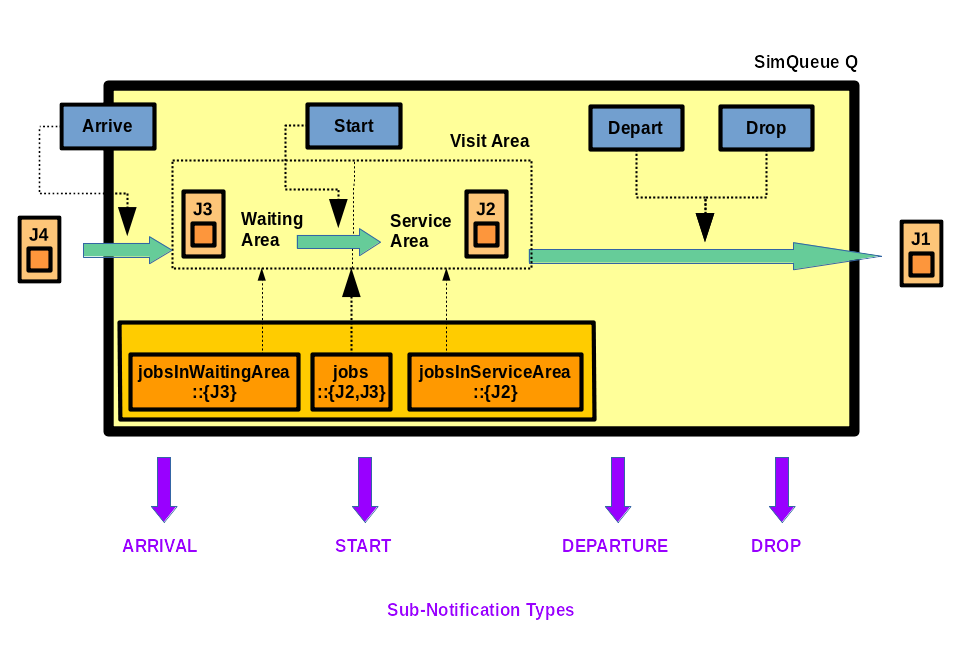
\includegraphics[width=\textwidth]{fig/ArriveDepartStartDrop}
\end{figure}

In the modified version of the figure,
  job \lstinline|J1| may have {\em departed\/}
  or have been {\em dropped\/} from \lstinline|Q|;
  the effect of either is the same on \lstinline|J1|,
  i.e., a job has no notion
  of having departed or having been dropped from its
  latest visited \lstinline|SimQueue|.
  
It is important to realize that the invocation
  of the \lstinline|Drop| operation
  is {\em always initiated by the queue during a visit\/};
  you cannot enforce it through an event on the event list,
  nor (directly) from an operation
  on the \lstinline|SimJob| in question.
Since by default,
  generic \lstinline|SimQueue|s
  have no reason to drop jobs,
  specific implementations that do
  must precisely specify
  (1) the conditions under which
  jobs are dropped
  and (2) the selection of which job is dropped
  once that condition is met.

The mechanism of dropping a job
  is present in many classical or
  more advanced queueing models.
The most common reason for dropping jobs
  is {\em lack of buffer space\/}:
A job arrives at a queueing system
  while all buffer space in that system
  has already been used for other
  visiting jobs.
The queueing system then resorts to dropping
  a single (in most cases) job.
Note that this may not be the arriving job!
The classical examples of systems that employ dropping
  jobs for lack of buffer space are the
  \lstinline|FCFS_B| (First-Come First-Served with Finite
  Buffer Size \lstinline|B|)
  and \lstinline|LCFS_B| (Last-Come First-Served with Finite
  Buffer Size \lstinline|B|) queues.
The former will drop an arriving job that finds
  a "full queue",
  in this case,
  that finds all available places in the waiting area
  occupied.
The latter, however,
  will drop the job in the waiting area
  with the earliest arrival time.
If no such job is present,
  i.e.,
  the system has zero buffer size,
  the arriving job is dropped instead.
  
A second reason for dropping jobs
  is a given limit on the job's {\em waiting time}.
In this case,
  a job is dropped from the waiting area
  once its time spent there
  exceeds some given threshold.
Many models with {\em impatient customers\/}
  fit this case.
Obvious variants put limits
  onto the {\em time spent in the service area}
  or onto the {\em sojourn time\/} of a job.
Combinations are also possible.
In \lstinline|jqueues|,
  you can actually turn {\em any\/}
  \lstinline|SimQueue|
  into one with impatient customers
  through the \lstinline|EncTL|
  {\em composite\/} queueing system implementation.
For more details,
  we refer to Section {\bf XXX}.
  
\section{The \texttt{\bf Revoke} Operation}
\label{sec:revoke}

Up to now,
  we have introduced job departures and drops
  as two means by which a \lstinline|SimJob|
  can end its visit to a \lstinline|SimQueue|.
Both are invoked at the discretion of the queue.
The third and final way
  in which a visit can end is through {\em revocation};
  the user-initiated exit of a job at a queue.
  
Revocations actually come in two flavors:
\begin{itemize}
	\item
	Users can invoke the external \lstinline|Revoke| operation,
	  requesting for the forced exit of a jobs.
	Every \lstinline|SimQueue| must support the operation.
	\item
	Users can set one or more conditions on a queue,
      or a combination of them,
      that trigger the automatic removal of the job
      once the condition is met.
	Such revocations are named {\em auto-revocations\/};
      we describe them in more detail
      in Section \ref{sec:auto-revocations}.
\end{itemize}

The external \lstinline|Revoke| operation
  {\em requests\/} the removal of a job visiting a queue.
In its most basic form,
  the so-called {\em unconditional revocation},
  this request cannot be denied by {\em any\/}
  \lstinline|SimQueue| implementation.
In other words,
  every \lstinline|SimQueue|
  supports unconditional revocation of a job.
After a job has been revoked,
  a \lstinline|REVOCATION| sub-notification is fired.
  
In Figure \ref{fig:ArriveDepartStartDropRevoke},
  we show the modified simple model of the state of
  a \lstinline|SimQueue|s
  and \lstinline|SimJob|s of Figure \ref{fig:ArriveDepartStartDrop},
  now including the \lstinline|Revoke| operation.

\begin{figure}[!htbp]
\label{fig:ArriveDepartStartDropRevoke}
\caption{Conceptual illustration
         of arrivals, departures, starts, drops and revocations
         at a \texttt{SimQueue}.}
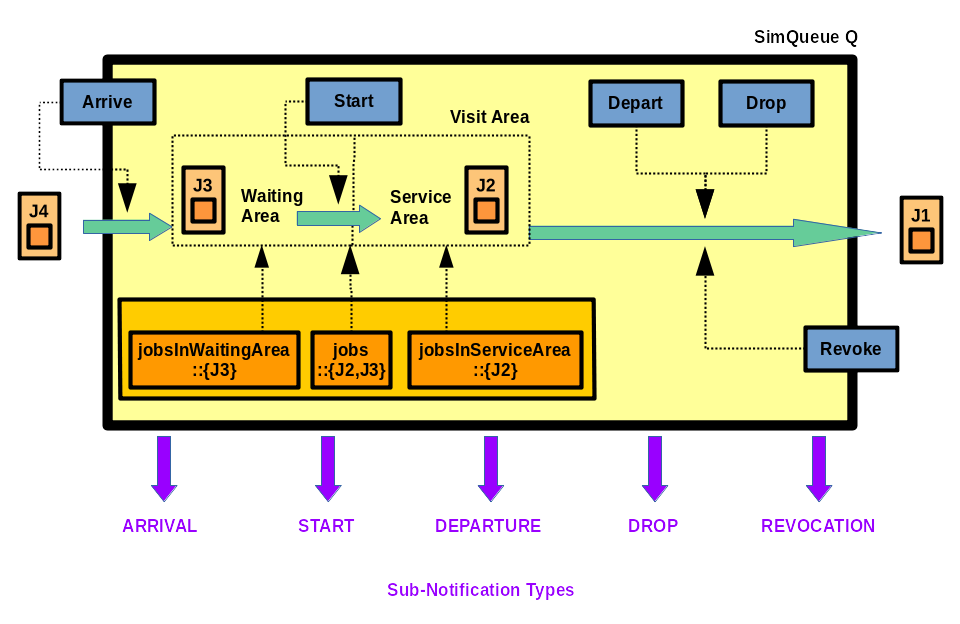
\includegraphics[width=\textwidth]{fig/ArriveDepartStartDropRevoke}
\end{figure}
  
In addition to the unconditional revocation,
  \lstinline|SimQueue| implementations
  may provide variants of the \lstinline|Revoke|
  operation that take an additional condition
  or combination of conditions on the state
  of the queue and/or job.
However,
  an invocation of such a {\em conditional\/}
  revocation cannot fail if
  the relevant condition is met

On every \lstinline|SimQueue|,
  the method \lstinline|revoke (double, SimJob)|
  revokes a job unconditionally from the queue.
The first argument is (as always)
  the simulation time of the request.
If the job is present a priori,
  the revocation request cannot fail;
  every \lstinline|SimQueue| implementation
  must honor it.
In the variant method
  \lstinline|revoke (double, SimJob, boolean)|,
  which is actually present on {\em any} \lstinline|SimQueue|,
  the third argument indicates
  whether it is allowed to revoke the job
  from the {\em service area}.
If the argument is \lstinline|false| and the job is indeed
  in the service area,
  the request will fail in a non-fatal way:
No revocation takes place and
  no sub-notification will be fired.
If, however, the job is in the waiting area,
  and/or the argument is set to \lstinline|true|
  and the job is present in either area,
  then, again, the request cannot fail.

\section{The \texttt{\bf AutoRevoke} Operation}
\label{sec:auto-revocations}

Auto-revocations are forced removals from a \lstinline|SimQueue|
  because a user-set condition on the queue is met.
The set of conditions for auto-revocation
  that can be set on a \lstinline|SimQueue|
  depends on the queue's type,
  however,
  every \lstinline|SimQueue|
  must have {\em any\/}
  auto-revocation condition
  {\em disabled by default}.
The only auto-revocation condition
  every \lstinline|SimQueue| {\em must\/}
  support, is the start of a job.
(But, it must be disabled by default.)
Auto-revocation is an internal operation
  name \lstinline|AutoRevoke|;
  the corresponding sub-notification is
  \lstinline|AUTO_REVOCATION|.

The condition(s) on a \lstinline|SimQueue|
  that trigger auto-revocation is captured
  in the queue's \lstinline|autoRevocationPolicy|
  property.
It is an essential property,
  meant to be set {\em only\/}
  immediately after construction or
  a \lstinline|Reset| invocation.
In Release 5 of \lstinline|jqueues|,
  the property has \lstinline|enum| type
  with possible values \lstinline|NONE|
  and \lstinline|UPON_START|.
With value \lstinline|NONE|,
  auto-revocation is essentially switched off.
  whereas with \lstinline|UPON_START|,
  {\em any\/} job that is about to start
  on a \lstinline|SimQueue| is automatically
  revoked.
  
In Figure \ref{fig:ArriveDepartStartDropRevokeAutoRevoke},
  we show the modified simple model of the state of
  a \lstinline|SimQueue|s
  and \lstinline|SimJob|s of Figure \ref{fig:ArriveDepartStartDropRevoke},
  now including the \lstinline|AutoRevoke| operation
  and the essential \lstinline|autoRevocationPolicy|
  property.

\begin{figure}[!htbp]
\label{fig:ArriveDepartStartDropRevokeAutoRevoke}
\caption{Conceptual illustration
         of arrivals, departures, starts,
         drops, revocations and auto-revocations
         at a \texttt{SimQueue}.}
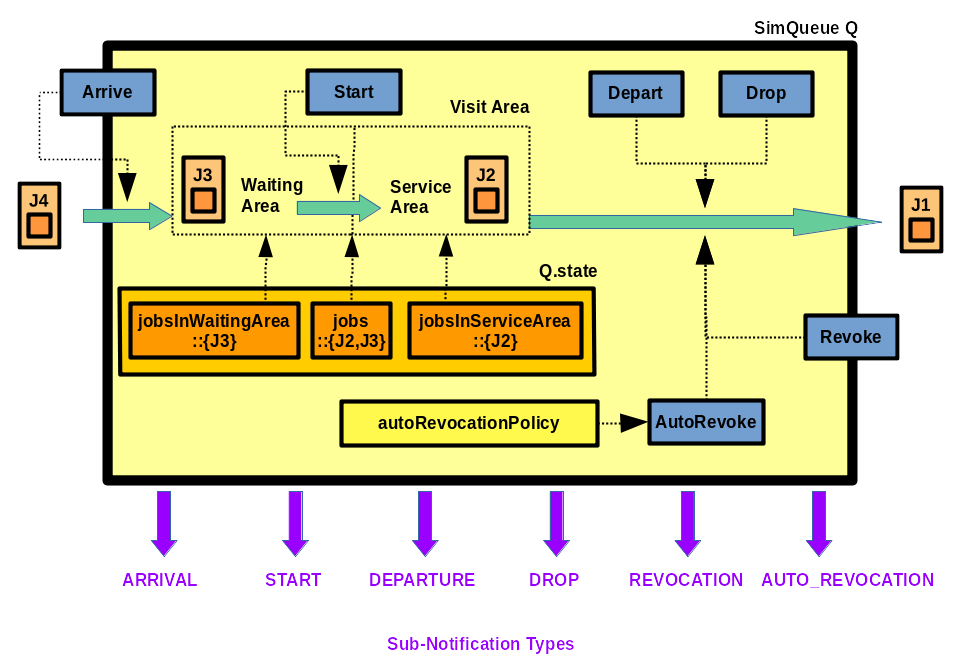
\includegraphics[width=\textwidth]{fig/ArriveDepartStartDropRevokeAutoRevoke}
\end{figure}
  
We do not expect many practical use cases
  requiring auto-revocations.
Moreover,
  we did not add the feature with specific use cases in mind;
  we merely needed the feature as a part of the
  {\em generic\/} \lstinline|SimQueue| interface
  in some of its specific implementations,
  in particular,
  the \lstinline|CTandem2| queueing system
  described in Section {\bf XXX}.
If at all possible,
  we advise against the use of auto-revocations
  and manipulation of
  the \lstinline|autoRevocationPolicy|
  property.
Then again,
  the concept is available on {\em any\/}
  \lstinline|SimQueue|,
  should you need it.
  
\section{QoS}
\label{sec:qos}

So far,
  we have introduced and described
  queueing systems
  that treat (or, distinguish, if you will)
  jobs based upon
  for instance their arrival time
  (\lstinline|FCFS|,
  \lstinline|LCFS|
  and derivatives),
  or their requested service time
  (\lstinline|SJF|
  and \lstinline|LJF|).
In so-called {\em multiclass queueing systems},
  jobs are (in addition) treated differently according to
  their membership to a {\em class\/} of jobs.
An easy example is the queueing system associated with
  checking in for an flight, with multiple quueues
  distinguishing between business-class passengers,
  and poor others.
Multi-class queueing systems are often referred to as
  {\em priority systems\/}
  or {\em QoS (Quality of Service) systems.}
In \lstinline|jqueues|,
  we mainly use the latter terminology,
  viz.,
  jobs belong to a {\em QoS class\/},
  in order to avoid name clashes
  with the Java \lstinline|class| concept.

Every \lstinline|SimQueue| and
  \lstinline|SimJob|
  possess two QoS-related
  essential properties,
  viz.,
  \lstinline|qosClass|
  and \lstinline|qosValue|.
On a \lstinline|SimQueue|,
  the \lstinline|qosClass| property
  holds the type
  (i.e., a \lstinline|Java|
   \lstinline|Class| object)
  the queue uses to distinguish 
  among jobs
  {\em for reasons of QoS}.
On a \lstinline|SimJob|,
  the property value holds the
  \lstinline|Java| \lstinline|class|
  the job uses to indicate its relative priority
  or its membership to a specific QoS class.
The actual object representing the priority
  of job class is held in the job's
  \lstinline|qosValue|.
This property also exists on
  every \lstinline|SimQueue|,
  but its semantics are {\em undefined\/}
  by default, and their
  \lstinline|qosValue| is therefore always
  \lstinline|null|.
  
The anticipated use cases are that:
\begin{itemize}
\item
  In a {\em non-QoS scenario},
    both \lstinline|qosClass|
    and \lstinline|qosValue|
    have their \lstinline|null|
    default values.
\item
  In a {\em QoS scenario},
    the \lstinline|qosClass| properties
    on jobs and queues must "match"
    and be non-\lstinline|null|;
    the matching refers to the requirement
    that \lstinline|qosClass| on the job
    must be an sub-class or implementation
    of \lstinline|qosClass| on the queue.
  The \lstinline|qosValue| property
    on the job holds the relative priority
    or job-class to which the job belongs;
    the value must be an object of type
    advertised by the job's \lstinline|qosClass|
    property, or a sub-class of it.
  The \lstinline|qosValue|
    on {\em any\/} queue is ignored and
    \lstinline|null|.
\end{itemize}
Somewhat unfortunately,
  there is a substantial number of corner cases
  that deviate from the two use cases above.
For instance,
  specific \lstinline|SimQueue| implementations
  feature special treatment of
  visiting \lstinline|SimJob|s
  with \lstinline|null|
  or incompatible value
  for their \lstinline|qosClass|
  property,
  or with a \lstinline|null| value
  for their \lstinline|qosValue|
  property.
We hope to describe these corner cases
  in a future version of this document,
  but for now we refer
  to the \lstinline|javadoc|
  specification for further details.

At this point,
  we have described {\em all\/}
  binary operations,
  internal as well as external,
  on \lstinline|SimJob| and \lstinline|SimQueue|.
In the next sections,
  we will describe operations, properties
  and sub-notification types specific
  {\em only\/} to \lstinline|SimQueue|.
   
\section{Queue-Access Vacations}
\label{sec:guided:qav}

In \lstinline|jqueues|, every queue,
  in other words, every \lstinline|SimQueue| implementation,
  {\em must\/} support the notion
  of so-called {\em queue-access vacations}.
During a queue-access vacation,
  {\em all arriving jobs are dropped},
  but jobs already visiting
  the queue are not affected.
In terms of queue state,
  every \lstinline|SimQueue| has a state
  property \lstinline|queueAccessVacation|
  of type \lstinline|boolean|
  that determines whether or not the
  queue is "on vacation".
Starting and stopping queue-access vacations
  is an external operation named \lstinline|SetQueueAccessVacation|,
  taking a \lstinline|boolean| argument
  to indicate whether the vacation starts or ends;
  the corresponding sub-notification types
  are \lstinline|QAV_START|
  and \lstinline|QAV_END|.
Be aware that these sub-notifications
  are {\em only\/} issued when the
  \lstinline|queueAccessVacation|
  property value
  {\em actually changes}.

In Figure \ref{fig:QueueAccessVacations},
  we show the modified simple model of the state of
  a \lstinline|SimQueue|s
  now including Queue-Access Vacations.

\begin{figure}[!htbp]
\label{fig:QueueAccessVacations}
\caption{\texttt{SimQueue} model with Queue-Access Vacations.}
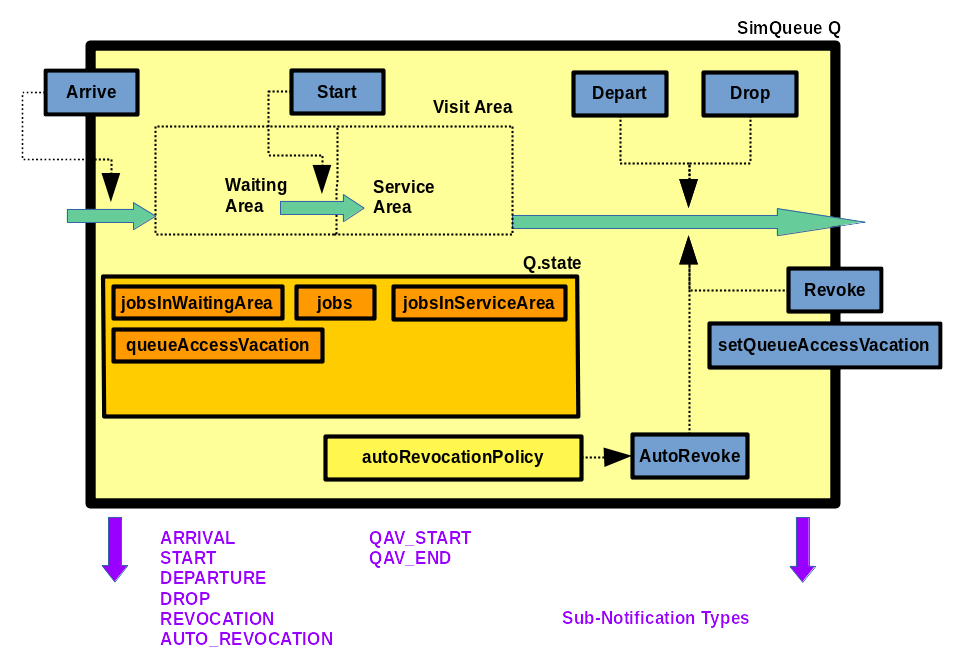
\includegraphics[width=\textwidth]{fig/QueueAccessVacation}
\end{figure}
  
\begin{sloppypar}
It is essential to note that queue-access vacations
  are {\em always\/} available to you
  as an independent means to drop arriving jobs
  because you think this is the right thing to do at this time.
In other words,
  \lstinline|SimQueue| implementations
  are {\em not\/} allowed to use the feature
  to get "their job done".
This turns the \lstinline|SetQueueAccessVacation|
  operation into a purely {\em external\/} one.
For instance,
  in our previous example with \lstinline|FCFS_B|,
  the queue {\em could\/} use queue-access vacations
  in order to drop jobs upon arrival
  if the buffer is full.
But, it is not allowed to do that,
  and it simply never touches
  the \lstinline|QueueAccessVacation| property.
\end{sloppypar}

Scheduling the start and end of queue-access vacations on a queue
  is easily achieved through the utility method
  \lstinline|SimQueueEventScheduler.scheduleQueueAccessVacation (SimQueue, double, boolean)|;
  the respective arguments being the queue to which the event applies,
  the scheduled time,
  and whether to start or end a queue-access vacation,
  respectively.
  
\section{Server-Access Credits}
\label{sec:guided:sac}

Every \lstinline|SimQueue| has the
  \lstinline|serverAccessCredits|
  state property of type \lstinline|int|,
  and setting its value is an
  external operation
  named \lstinline|SetServerAccessCredits|.
The value represents the maximum number of
  jobs on that particular \lstinline|SimQueue|
  that can \lstinline|START|,
  in other words,
  move from the waiting area into
  the service area
  as explained in Section \ref{sec:guided:wait-serv-area}.
Whenever a job starts,
  the \lstinline|serverAccessCredits| value
  is decremented with one,
  and if it reaches zero,
  jobs are no longer allowed to start.
However,
  the \lstinline|serverAccessCredits| value
  {\em never\/}
  affects jobs that are already in the
  service area.

\begin{sloppypar}
Every \lstinline|SimQueue| reports
  changes to {\em the availability of server-access credits\/}
  (i.e., not just changes to the actual value)
  through the \lstinline|LOST_SAC|
  and \lstinline|REGAINED SAC|
  notification.
The former notification can be the result of
  starting one or more jobs
  {\em or\/}
  the invocation of \lstinline|SetServerAccessCredits|
  with argument zero,
  whereas the latter notification is always
  the result of \lstinline|SetServerAccessCredits|
  with argument (at least) non-zero.
\end{sloppypar}

In Figure \ref{fig:ServerAccessCredits},
  we show the modified simple model of the state of
  a \lstinline|SimQueue|s
  now including Server-Access Credits.

\begin{figure}[!htbp]
\label{fig:ServerAccessCredits}
\caption{\texttt{SimQueue} model with Server-Access Credits.}
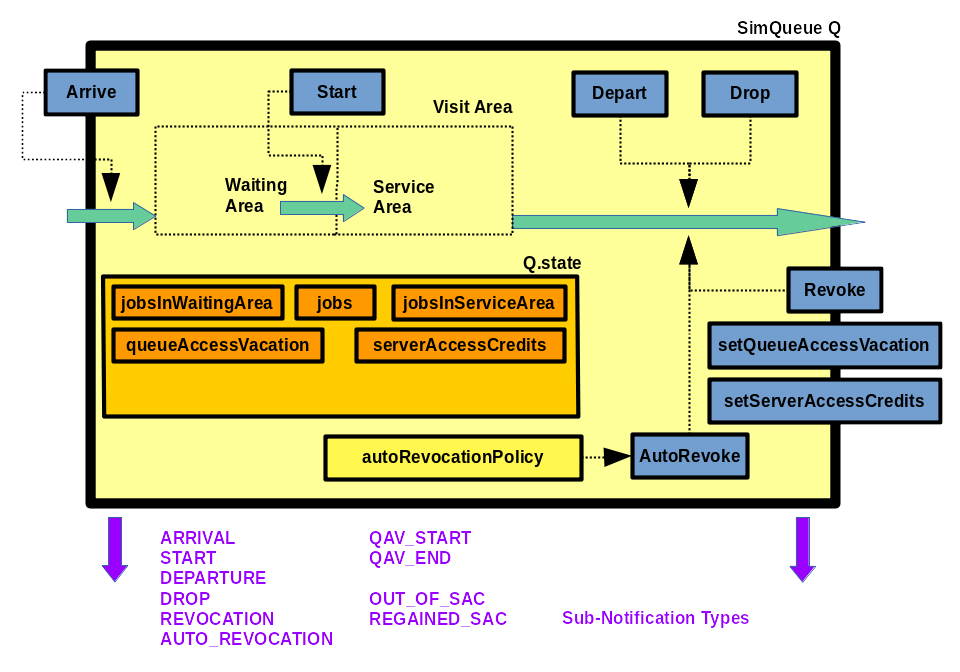
\includegraphics[width=\textwidth]{fig/ServerAccessCredits}
\end{figure}

Since the number
  \lstinline|serverAccessCredits|
  of server-access credits is integral,
  it is represented by \lstinline|Java|'s
  \lstinline|int| simple type,
  but the value
  \lstinline|Integer.MAX_VALUE|
  is interpreted as infinity.
This is in fact the default value;
  and as long as \lstinline|ServerAccessCredits|
  has this value,
  it is not affected by starting jobs
  (the value is not decremented),
  effectively turning off the mechanism of
  server-access credits.

\begin{sloppypar}
In addition to the default value being $\infty$,
  \lstinline|SimQueue| implementations
  cannot use \lstinline|ServerAccessCredits|
  to meet their requirements.
For instance, in order to implement queueing
  systems with multiple servers like
  \lstinline|FCFS_c|
  (see Section \ref{sec:FCFS_c}),
  the use of
  \lstinline|ServerAccessCredits|
  could be queue handy.
However, decreasing the value upon \lstinline|START|
  of a job is the only thing queues may do
  (and must adhere to).
\end{sloppypar}

These two facts imply that
  if you never "touch"
  the \lstinline|serverAccessCredits|
  property value
  through the use of the
  \lstinline|SetServerAccessCredits| operation,
  you can safely forget the entire concept.
On the other hand,
  should you have any need for it,
  it is always available,
  whatever the (concrete) queue type.

\section{The \texttt{startArmed} State Property}
\label{sec:start-armed}

Every \lstinline|SimQueue| (implementation)
  supports the \lstinline|boolean|
  \lstinline|startArmed| state property;
  its changes are reported
  with \lstinline|STA_TRUE|
  and \lstinline|STA_FALSE|,
  respectively.
In Figure \ref{fig:StartArmed},
  we show the modified simple model of the state of
  a \lstinline|SimQueue|s
  now including the \lstinline|startArmed|
  state property.

\begin{figure}[!htbp]
\label{fig:StartArmed}
\caption{\texttt{SimQueue} model with \texttt{startArmed} state property.
         (Full model of a \texttt{SimQueue}.)}
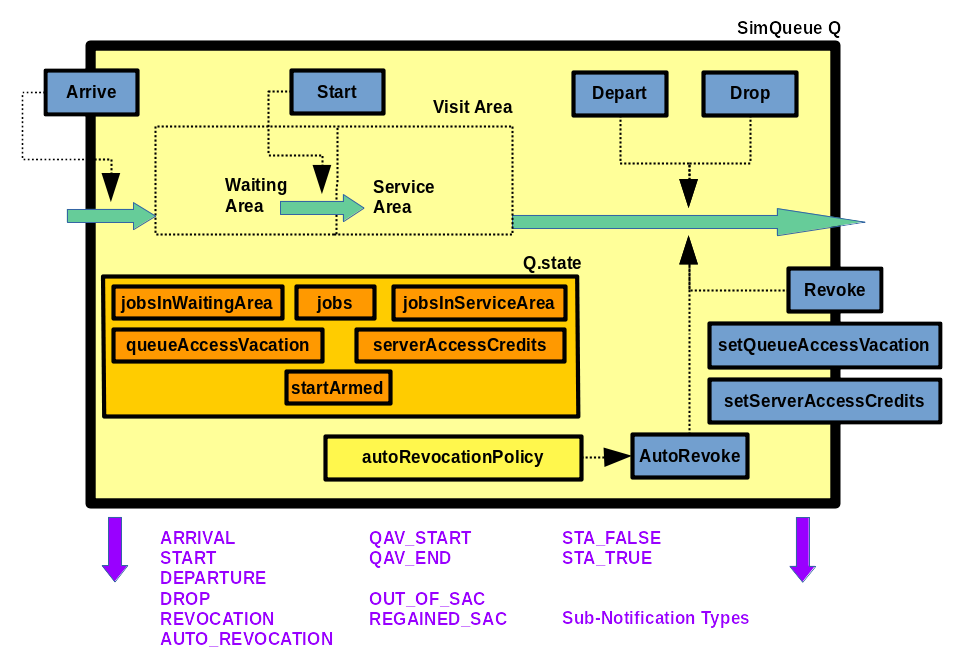
\includegraphics[width=\textwidth]{fig/StartArmed}
\end{figure}

\begin{sloppypar}
The \lstinline|startArmed|
  property is a but difficult to grasp at first sight
  and has little use in simulations,
  but it is essential in so-called {\em compressed tandem queues},
  in particular \lstinline|CTandem2|,
  see Section {\bf XXX}.
Nonetheless,
  since it is part of the \lstinline-SimQueue- interface,
  we state its formal definition:
A \lstinline-SimQueue- has state
  property \lstinline-startArmed == true-
  if and only if {\em any\/} (hypothetical)
  arriving job
  {\em would\/} start service immediately
  (i.e., enter the service area upon arrival immediately),
  {\em if\/} the following conditions {\em would\/} hold:
\begin{itemize}
\item the absence of a queue access vacation,
\item at least one server-access credit, and
\item an empty waiting area. 
\end{itemize}
The actual values of these three state properties is irrelevant,
  which, admittedly, makes the definition quite hard to understand.
If a \lstinline-SimQueue- has \lstinline-startArmed == true-,
  changing its state such that it meets the three conditions above,
  would lead to the immediate start of a hypothetical arriving job
  (irrespective of the type and properties of that job).
\end{sloppypar}

As an example, consider an instance of the
  (single-server) \lstinline-FCFS- queueing system
  which has no queue-access vacation,
  and suppose that it is out of server-access credits,
  has a single job in the waiting area
  and no jobs in the service area.
In this case, \lstinline-startArmed == true- because
  an arriving job would be taken into service
  if we apply the state transformation rules:
  (1) remove any queue-access vacation (check),
  (2) give it a single (or more) server-access credit,
  and (3) remove the job from the waiting area.
This leaves a \lstinline-FCFS- queueing system without
  queue-access-vacation, no jobs in the waiting area,
  and at least one server-access credits,
  and surely, such a queue would immediately start an arriving job.
If initially, however, a job would be in service at the queue,
  we have \lstinline-startArmed == false-,
  because the transformed state of the queueing system has
  a job in service,
  and \lstinline-FCFS- cannot guarantee at all that
  an arriving job would be taken into service.
If on he other side, in the latter case
  the queue is of type \lstinline-PS-,
  we would have \lstinline-startArmed == true-,
  because the presence of jobs in the service area in \lstinline-PS-,
  does not inhibit it from immediately starting newly arrived jobs.
 
Informally, the \lstinline-startArmed- state property of a queue
  reflects the fact {\em as far as the service area is concerned},
  at least one more job can be added to it {\em immediately}.
  
With the introduction of the \lstinline|startArmed| property,
  our model of a \lstinline|SimQueue| is now complete.

\section{The Requested Service Time of a Job}
\label{sec:requested-service-time}

So far we have not been concerned
  with the time it takes to serve a job until completion,
  if a \lstinline|SimQueue| supports the notion
  of "serving jobs".
Well, in \lstinline|jqueues|,
  the default behavior is that
  a queue interrogates the job for its
  {\em requested service time}.
To that purpose,
  each \lstinline|SimJob| has the
  \lstinline|requestedServiceTimeFunction|
  essential property,
  which has type \lstinline|Function<SimQueue, Double>|.
Its value returns a {\em requested service time\/}
  for each \lstinline|SimQueue| argument.

Compared to the \lstinline|SimQueue| interface,
  the \lstinline|SimJob| interface is remarkably simple.
Apart from the internal maintenance of the \lstinline-SimQueue-
  being visited,
  a \lstinline-SimJob- only needs to provide information on the
  so-called {\em requested service time\/} for a queue visit,
  through implementation of
  \lstinline-getServiceTime (Q)-.
This method is used
  by a \lstinline|SimQueue|
  to query the requested service time,
  and appropriately schedule a departure event for the job,
  but it can be called anytime.
However,
  the returned value
  should not change during a visit to a \lstinline-SimQueue-,
  and it is not manipulated by the queue being visited,
  in other words,
  it cannot be used
  to query the remaining service time
  of a job at a queue.
It is safe though
  to change the return value in-between queue visits.
However, the convention is
  that the method then returns
  the required service time
  at the {\em next} visit to the queue.
For instance,
  many test and job-factory classes depend on this,
  as they often directly probe
  a non-visiting job
  for its required service time at a queue.
Obviously, implementations
  must be prepared
  for invocations
  of this method while not visiting a queue.
If \lstinline|null| is passed as argument
  the service time at the current queue is used,
  or zero if the job is not currently visiting a queue.

\section{The \texttt{DefaultSimjob} Class}

The \lstinline|DefaultSimJob| provides a reasonable
  initial implementation of \lstinline|SimJob|.
It features two constructors,
  both of which take the event list (may be \lstinline|null|)
  and the name of the job (may be \lstinline|null|)
  as argument.
The first,

\begin{lstlisting}[
  basicstyle=\tiny]
  public DefaultSimJob (final SimEventList eventList, final String name, final Map<Q, Double> requestedServiceTimeMap)
\end{lstlisting}

\noindent takes as additional argument
  a \lstinline|Map|
  from \lstinline|Q| onto requested
  service times,
  allowing different values
  on a per-\lstinline|SimQueue| basis.
The second,

\begin{lstlisting}[
  basicstyle=\tiny]
  public DefaultSimJob (final SimEventList eventList, final String name, final double requestedServiceTime)
\end{lstlisting}

\noindent takes a \lstinline|double| as third argument
  holding the requested service time at {\em any\/}
  \lstinline|SimQueue|.

\section{Summary of Properties}

In Table
  \ref{SimJob_Properties}
  we list the (mandatory) properties
  of a \lstinline|SimJob|.
The table starts with a specification of
  the super type of \lstinline|SimJob|,
  viz., \lstinline|SimEntity|.
We consistently try to always
  specify the super type in
  tables showing properties, operations,
  etc., merely as a reminder to the reader
  that such a table actually {\em augments\/}
  the corresponding table from the super type.
  
\begin{table}[!htbp]
\caption{Mandatory properties of a \lstinline|SimJob|.}
\label{SimJob_Properties}
\begin{center}
\begin{tabular}{|l|l|l|}
\hline
{\bf Name} & {\bf Type} & {\bf Default/Reset} \\
\hline
\multicolumn{3}{|c|}{} \\
\multicolumn{3}{|c|}{\lstinline[basicstyle=\large]{SimJob}} \\
\multicolumn{3}{|c|}{} \\
\hline
\multicolumn{3}{|c|}{} \\
\multicolumn{3}{|c|}{\bf Super} \\
\multicolumn{3}{|c|}{} \\
\hline
\multicolumn{2}{|l|}{\lstinline|SimEntity|}
  & See Table \ref{SimEntity_Properties}.
  \\
  \hline
\multicolumn{3}{|c|}{} \\
\multicolumn{3}{|c|}{\bf State Properties} \\
\multicolumn{3}{|c|}{} \\
\hline
\lstinline|queue|
  & \lstinline|SimQueue|
  & \lstinline|null|.
  \\
  \hline
\multicolumn{3}{|c|}{} \\
\multicolumn{3}{|c|}{\bf Essential Properties} \\
\multicolumn{3}{|c|}{} \\
\hline
\lstinline|qosClass|
  & \lstinline|Class|
  & \lstinline|null|.
  \\
  \hline
\lstinline|qosValue|
  & \lstinline|Object|
  & \lstinline|null|.
  \\
  \hline
\lstinline|requestedServiceTimeFunction|
  & \lstinline|Function<SimQueue, Double>|
  & \lstinline|q->1.0;|
  \\
  \hline
\multicolumn{3}{|c|}{} \\
\multicolumn{3}{|c|}{\bf Cosmetic Properties} \\
\multicolumn{3}{|c|}{} \\
\hline
\multicolumn{3}{|l|}{None.} \\
\hline
\end{tabular}
\end{center}
\end{table}
  
The only mandatory state property
  on a \lstinline|SimJob|
  is the \lstinline|queue| property
  which holds
  the \lstinline|SimQueue|
  currently being visited by the \lstinline|SimJob|.
The mandatory reset value is \lstinline|null|,
  as shown in the third column,
  meaning that (1) a job cannot visit a queue
  "upon construction", and (2)
  visits to queues end upon a \lstinline|Reset|.

A \lstinline|SimJob|'s essential properties
  are the two QoS-related properties
  \lstinline|qosClass| and \lstinline|qosValue|
  described in Section \ref{sec:qos},
  and the \lstinline|requestedServiceTimeFunction|
  described in Section \ref{sec:requested-service-time}.
Be aware that for essential (and cosmetic) properties
  the third column holds the property's {\em default\/}
  value,
  and that the value of such properties can {\em only\/}
  be set upon construction or {\em immediately\/}
  after a \lstinline|Reset|,
  {\em unless stated otherwise}.
Also,
  the value of an essential property typically
  survives a \lstinline|Reset|.
In the case of \lstinline|SimJob|,
  all essential properties actually
  can be set safely {\em in between visits\/}
  as well.
A \lstinline|SimJob| has no specific
  {\em cosmetic\/} properties.
   
In Table
  \ref{SimQueue_Properties}
  we list the (mandatory) properties
  of a \lstinline|SimQueue|.
  
\begin{table}[!htbp]
\caption{Mandatory properties of a \lstinline|SimQueue|.}
\label{SimQueue_Properties}
\begin{center}
\begin{tabular}{|l|l|l|}
\hline
{\bf Name} & {\bf Type} & {\bf Default/Reset} \\
\hline
\multicolumn{3}{|c|}{} \\
\multicolumn{3}{|c|}{\lstinline[basicstyle=\large]{SimQueue}} \\
\multicolumn{3}{|c|}{} \\
\hline
\multicolumn{3}{|c|}{} \\
\multicolumn{3}{|c|}{\bf Super} \\
\multicolumn{3}{|c|}{} \\
\hline
\multicolumn{2}{|l|}{\lstinline|SimEntity|}
  & See Table \ref{SimEntity_Properties}.
  \\
  \hline
\multicolumn{3}{|c|}{} \\
\multicolumn{3}{|c|}{\bf State Properties} \\
\multicolumn{3}{|c|}{} \\
\hline
\lstinline|jobs|
  & \lstinline|Set<SimJob>|
  & Empty \lstinline|Set|.
  \\ \hline
\lstinline|jobsInWaitingArea|
  & \lstinline|Set<SimJob>|
  & Empty \lstinline|Set|
  \\ \hline
\lstinline|jobsInServiceArea|
  & \lstinline|Set<SimJob>|
  & Empty \lstinline|Set|.
  \\
  \hline
\lstinline|queueAccessVacation|
  & \lstinline|boolean|
  & \lstinline|false|.
  \\
  \hline
\lstinline|serverAccessCredits|
  & \lstinline|int|
  & \lstinline|Integer.MAX_VALUE|
  \\
  &
  & ("$=$" $\infty$).
  \\ \hline
\lstinline|startArmed|
  & \lstinline|boolean|
  & Depends (only) \\
  &
  & on sub-type. \\ \hline
\multicolumn{3}{|c|}{} \\
\multicolumn{3}{|c|}{\bf Essential Properties} \\
\multicolumn{3}{|c|}{} \\
\hline
\lstinline|autoRevocationPolicy|
  & \lstinline|AutoRevocationPolicy|
  & \lstinline|NONE|.
  \\
  \hline
\lstinline|qosClass|
  & \lstinline|Class|
  & \lstinline|null|.
  \\
  \hline
\lstinline|qosValue|
  & \lstinline|Object|
  & \lstinline|null|.
  \\
  \hline
\multicolumn{3}{|c|}{} \\
\multicolumn{3}{|c|}{\bf Cosmetic Properties} \\
\multicolumn{3}{|c|}{} \\
\hline
\multicolumn{3}{|l|}{None.} \\
\hline
\end{tabular}
\end{center}
\end{table}

Since \lstinline|SimQueue| extends \lstinline|SimEntity|,
  the table starts with a specification of the super type
  and a reference to the specification of
  \lstinline|SimEntity|'s properties.
The three visit-related state properties
  on a \lstinline|SimQueue|
  are \lstinline|jobs|,
  \lstinline|jobsInWaitingArea|
  and \lstinline|jobsInServiceArea|;
  note that
  {\em the former
       is always the disjoint union
       of the latter two}.
In addition, any \lstinline|SimJob|
  \lstinline|j| present in
  either set
  on some \lstinline|SimQueue| \lstinline|q|
  must necessarily have
  \lstinline|j.queue == q|.
  
The remaining state properties are not
  (directly) related to job visits;
  they are specific to \lstinline|SimQueue|.
The \lstinline|queueAccessVacation| property
  indicates whether or not the \lstinline|SimQueue|
  is on queue-access vacation
  as explained in Section \ref{sec:guided:qav}.
The \lstinline|serverAccessCredits| property
  holds the remaining number of jobs
  allowed to start (in absence of events
  changing the property).
It is explained in more detail
  in Section \ref{sec:guided:sac}.
The value \lstinline|Integer.MAX_VALUE|
  is interpreted in this context as infinity:
If the property holds this value,
  it is not decremented
  upon the start of a job.
We repeat the remark that
  both the \lstinline|queueAccessVacation|
  and \lstinline|serverAccessCredits|
  properties
  are always fully available to the user
  on {\em any\/} \lstinline|SimQueue|
  implementation;
  they are {\em never\/}
  (to be) used for internal purposes. 
Finally,
  the \lstinline|startArmed| property
  indicates whether or not,
  sloppily put,
  the service area would immediately
  admit {\em any\/} arriving job
  in the hypothetical case that
  the queue is (1) not on server-access vacation,
  (2) has at least one server-access credit
  and (3) has an empty waiting area.
It is explained in detail in Section \ref{sec:start-armed}.

The mandatory cosmetic properties on a \lstinline|SimQueue|
  are \lstinline|autoRevocationPolicy|
  explained in Section \ref{sec:auto-revocations},
  and the QoS-related properties
  \lstinline|qosClass| and \lstinline|qosValue|
  explained in Section \ref{sec:qos}.
We repeat the remark that cosmetic
  properties can be changed from user code
  {\em anytime}.

\section{Summary of Operations}
         
In Table \ref{tab:guided:operations},
  we summarize the operations supported on a \lstinline|SimQueue|,
  subdivided into \lstinline|SimEntity|
  and \lstinline|SimQueue| operations.

\begin{table}[!htbp]
	\label{tab:guided:operations}
	\caption{The operations on a \texttt{SimQueue}.}
	\begin{center}
%		\begin{longtabu}{|l|l|l|}
		\begin{tabular}{|l|l|l|}
			\hline
			\multicolumn{3}{|c|}{} \\
			\multicolumn{3}{|c|}{\texttt{SimEntity} Operations} \\
			\multicolumn{3}{|c|}{} \\
			\hline
			\lstinline|Reset|   & E & \lstinline|double newTime| \\ \hline
			\lstinline|Update|  & E & \lstinline|double newTime| \\ \hline
			\hline
			\multicolumn{3}{|c|}{} \\
			\multicolumn{3}{|c|}{\texttt{SimJQ} Operations} \\
			\multicolumn{3}{|c|}{} \\
			\hline
			\lstinline|Arrive|            & E & \lstinline|double time|, \lstinline|SimJob|, \lstinline|SimQueue| \\ \hline
			\lstinline|Drop|              & I & \lstinline|double time|, \lstinline|SimJob|, \lstinline|SimQueue| \\ \hline
			\lstinline|Revoke|            & E & \lstinline|double time|, \lstinline|SimJob|, \lstinline|SimQueue|,\\
			&   & \lstinline|boolean interruptService|                              \\ \hline
			\lstinline|AutoRevoke|        & I & \lstinline|double time|, \lstinline|SimJob|, \lstinline|SimQueue| \\ \hline
			\lstinline|Start|             & I & \lstinline|double time|, \lstinline|SimJob|, \lstinline|SimQueue| \\ \hline
			\lstinline|Depart|            & I & \lstinline|double time|, \lstinline|SimJob|, \lstinline|SimQueue| \\ \hline
			\hline
			\multicolumn{3}{|c|}{} \\
			\multicolumn{3}{|c|}{\texttt{SimQueue} Operations} \\
			\multicolumn{3}{|c|}{} \\
			\hline
			\lstinline|SetQueueAccessVacation| & E & \lstinline|double|, \lstinline|SimQueue|, \lstinline|boolean| \\ \hline
			\lstinline|SetServerAccessCredits| & E & \lstinline|double|, \lstinline|SimQueue|, \lstinline|int|     \\ \hline
%		\end{longtabu}
		\end{tabular}
	\end{center}
\end{table}

The first column in the table shows the name of the operation.
Note that subtle change in naming between
  a {\em notification\/} (like \lstinline|ARRIVAL|)
  and its corresponding {\em operation\/} (like \lstinline|Arrive|).
The second column indicates whether the operation
  is External (E) or Internal (I).
Note that with the exception of \lstinline|Update|,
  an external operation on a \lstinline|SimEntity|
  is {\em never\/} invoked from within the entity itself.
The third column provides the arguments to the operation,
  without going into the details of the method prototypes.
The argument names are only shown when needed for clarification;
  for most arguments, the type is self-explanatory.

\section{Summary of Sub-Notification Types}

In Table \ref{tab:guided:sub-notification-types},
  we summarize the notification types supported on a \lstinline|SimQueue|,
  subdivided into \lstinline|SimEntity|, \lstinline|SimJQ|
  and \lstinline|SimQueue| notification types.
The \lstinline|SimEntity| notification types
  apply to any \lstinline|SimEntity|,
  the \lstinline|SimJQ| types to \lstinline|SimJob|s and \lstinline|SimQueue|s,
  and the \lstinline|SimQueue| types to \lstinline|SimQueue|s only.

\begin{table}[!htbp]
	\label{tab:guided:sub-notification-types}
	\caption{The sub-notification types from a
             \texttt{SimJob} and \texttt{SimQueue}.}
	\begin{center}
%		\begin{longtabu}{|l|l|}
		\begin{tabular}{|l|l|}
			\hline
			\multicolumn{2}{|c|}{} \\
			\multicolumn{2}{|c|}{\lstinline[basicstyle=\ttfamily]{SimJQ} Sub-Notification Types} \\
			\multicolumn{2}{|c|}{(Common to \lstinline[basicstyle=\ttfamily]{SimJob}
            and \lstinline[basicstyle=\ttfamily]{SimQueue})} \\
			\multicolumn{2}{|c|}{} \\
			\hline
			\lstinline|ARRIVAL|            & \lstinline|double time|, \lstinline|SimJob|, \lstinline|SimQueue| \\ \hline
			\lstinline|DROP|               & \lstinline|double time|, \lstinline|SimJob|, \lstinline|SimQueue| \\ \hline
			\lstinline|REVOCATION|         & \lstinline|double time|, \lstinline|SimJob|, \lstinline|SimQueue| \\ \hline
			\lstinline|AUTO_REVOCATION|    & \lstinline|double time|, \lstinline|SimJob|, \lstinline|SimQueue| \\ \hline
			\lstinline|START|              & \lstinline|double time|, \lstinline|SimJob|, \lstinline|SimQueue| \\ \hline
			\lstinline|DEPARTURE|          & \lstinline|double time|, \lstinline|SimJob|, \lstinline|SimQueue| \\ \hline
			\hline
			\multicolumn{2}{|c|}{} \\
			\multicolumn{2}{|c|}{\lstinline[basicstyle=\ttfamily]{SimQueue} (Specific) Sub-Notification Types} \\
			\multicolumn{2}{|c|}{} \\
			\hline
			\lstinline|QAV_START|    & \lstinline|double time|, \lstinline|SimQueue| \\ \hline
			\lstinline|QAV_END|      & \lstinline|double time|, \lstinline|SimQueue| \\ \hline
			\lstinline|OUT_OF_SAC|   & \lstinline|double time|, \lstinline|SimQueue| \\ \hline
			\lstinline|REGAINED_SAC| & \lstinline|double time|, \lstinline|SimQueue| \\ \hline
			\lstinline|STA_FALSE|    & \lstinline|double time|, \lstinline|SimQueue| \\ \hline
			\lstinline|STA_TRUE|     & \lstinline|double time|, \lstinline|SimQueue| \\ \hline
%		\end{longtabu}
        \end{tabular}
	\end{center}
\end{table}

The first column is the name of the sub-notification type
  as it appears in (for instance) the output of
  several \lstinline|SimEntityListener|
  implementations.
The second column provides the arguments
  that are supplied with the notification type;
  and only if needed for clarity, the argument is named.
This column, however,
  is merely provided so you understand the meaning of the
  arguments in the output
  and in the code;
  it does not provide literal lists of arguments to any method.
But it should, for instance, allow you
  to look up the \lstinline|javadoc|
  for a specific \lstinline|SimEntityListener|,
  and known which methods to override,
  and what their arguments mean.
Recall that a state change is reported
  atomically
  as a \lstinline|List| of sub-notifications.